\documentclass[11pt,a4paper,DIV=10,]{scrartcl}
%\usepackage[latin1]{inputenc}
\usepackage[utf8]{inputenc}
\usepackage{lmodern}
\usepackage[ngerman]{babel}
\usepackage{amsmath}
\usepackage{amsfonts}
\usepackage{amssymb}
\usepackage{fancybox}
\usepackage{multicol}
\usepackage{graphicx}
\usepackage{color}
\usepackage{colortbl}
% Define user colors using the RGB model
\definecolor{dunkelgrau}{rgb}{0.8,0.8,0.8}
\definecolor{hellgrau}{rgb}{0.95,0.95,0.95}
\usepackage{booktabs}
\usepackage[normal,font={small,color=black}, labelfont=bf,figurename=Abb.]{caption}
\usepackage{float}
\usepackage{cite}
\usepackage{url}
\bibliographystyle{unsrtnat}
\usepackage[numbers]{natbib}
\usepackage[T1]{fontenc}
%
\begin{document}
\onecolumn
\subsection*{Versuchsprotokoll zum 1. Kurstag }
\section*{Zum Wasserhaushalt von Pflanzen -- Bestimmung des Wasserpotentials, des osmotischen Potentials  und des Druckpotentials bei \textit{Solanum Tuberosum}}
\textbf{Christoph van Heteren-Frese\footnotemark[1], Jana Jerosch\footnotemark[1], Nora Pauli\footnotemark[1]} \\[0.1cm]
\footnotemark[1]Freie Universität Berlin\\[0.2cm]
Eingereicht am 13.11.2012\\
\hrule
%
\section*{Einleitung}    
%Das vorliegende Protokoll wurde von den Autoren im Rahmen des pflanzenphysiologischen Grundpraktikums als Bestandteil des Moduls \textit{Physiologie und Biochemie der Pflanzen und Tiere} der Freien Universität Berlin verfasst. 
Der Wasseraustausch von Zellen findet überwiedend durch \textbf{Osmose} statt, bei der Wasser durch eine semipermeable Membran\footnote{Eine semipermeable (selektiv permeable) Membran ist für in Wasser gelösten Stoffe nur schwer durchlässig bzw. gänzlich undruchlässig. Eine \textbf{biologische Membran} stellt eine solche Membran dar.}  entlang eines chemischen Gradienten fließt; von der Lösung mit der niedrigeren Stoff\-konzentration in die Lösung mit der höheren Stoff\-konzentration. Dieses Prinzip bildet die Grundlage für den hier diskutierten Versuch, bei dem sowohl das Wasserpotential als auch das osmotische Potential von \textit{Solanum Tuberosum} in je einem Teilversuch bestimmt wurde. Aufgrund dieser Werte wurde das Druckpotential rechnerisch ermittelt.
\subsection*{Wasserpotential}
Als Wasserpotential\footnote{Der Wortteil \textit{potential} bezieht sich auf die potentielle Energie des Wassers, also seine Fähigkeit Arbeit zu verrichten. Dies kann z.B. zur Ausdehnung der Zelle führen.} bezeichnet man die Kapazität einer Zelle Wasser durch Osmose
aufzunehmen. Die hierfür verwendete Einheit ist der Druck (Pascal). Das Wasserpoten-
zial ist somit eine Kenngröße, durch die der Wassergehalt von Zellen charakterisiert
werden kann. Zudem können Aussagen über die Richtung von Wasserbewegungen gemacht werden. Dabei ist das Wasserpotential $\Psi_w$ definiert als das chemische Potential des
Wassers in Bezug zu einen Grundzusdstand (reines Wasser) pro Molvolumen:
\begin{equation}
\Psi=\dfrac{\mu_{H_2O}-\mu^0_{H_2O}}{\overline{V}_{H_2O}}
\end{equation}
Grundsätzlich bewegt sich freies Wasser vom Ort des höheren Wasserpotenzials zum Ort des
niedrigeren Wasserpotenzials. Ist das Wasserpotenzial an beiden Orten gleich, findet
\textbf{kein} Wasserfluss statt. \citep[vgl.][S. 52]{schopfer_pflanzenphysiologie_2010}
\subsection*{Osmotisches Potential}
Nach Van't Hoff ist das Osmotische Potential (osmotischer Druck) einer Lösung:
\begin{equation}
\Psi_S=c\cdot R\cdot T \label{hoff}
\end{equation}
Das osmotische Potential  ergibt sich demnach aus der Summe der gelösten Teilchen, der Temperatur soiwe der Gaskonstante. 
%
\section*{Material und Methoden}
\subsection*{Material}
\begin{enumerate}
	\item[•] 1 Kartoffel (\textit{Solanum Tuberosum})
	\item[•] Saccharose-Stammlösung (1 Mol)
	\item[•] Waage
	\item[•] Osmometer
\end{enumerate}
\subsection*{Kompenssationsmethode}
Die Bestimmung des Wasserpotentials geschah mit Hilfe der Kompensationsmethode. Hier\-zu  wurden Gewebesegmente bekannten Gewichts in Saccharoselösungen unter\-schied\-lichen Wasserpotenzials gegeben und nach drei Studen erneut gewogen. Durch an\-schließ\-en\-de Ermittlung der Gewichtsveränderung liesen sich Rückschlüsse auf das Wasserpotentials des Gewebes ziehen \citep[vgl.][S. 261]{strasburger_lehrbuch_2012}.
\subsection*{Kryoskopie}
Das osmotische Potential wurde durch eine kryoskopische Messung bestimmt. Die Metho\-de basiert auf der  Gefrierpunkterniedrigung eines Lösungsmittels durch Zugabe von löslichen Substanzen. Das Maß der Erniedrigung des Gefrierpunktes steht hierbei in Verbindung mit der Konzentration des zugesetzten Stoffes, so dass dies Rückschlüsse auf die Konzentration der Probe erlaubt \citep[vgl.][S. 261]{strasburger_lehrbuch_2012}.
%
\section*{Durchführung}
Für die Bestimmung des Wasserpotentials wurde aus der Saccharose-Stammlösung eine Verdünnungsreihe erstellt und in fünf Petrischalen gegeben (Konzentrationen siehe Tabelle \ref{tab1}). Ein Teil der Kartoffel wurde in Würfel von ca. $5\times5\times5$ mm Kantenlänge geschnitten und anschließend in Portionen von jeweils ca. fünf Gramm in die unterschiedlich konzentrierte Sacharose-Lösung gegeben. Nach drei Stunden wurden die Gewebeproben aus der Lösung genommen und gewogen.

Für die Bestimmung des osmotischen Potentials wurde der Rest der Kartoffel zerrieben, durch ein Stück Mull gepresst und mehrfach zentrifugiert. Der so enstandtende Zellsaft wurde mit einem Osmometer analysiert.
%
\section*{Ergebnisse}
\subsection*{Wasserpotential}
Die Ergbnisse des ersten Teilversuches zur Bestimmung des Wasserpotentials sind in Tabelle 1 und Abbildung 1 dargestellt.
\begin{table}[H]
\caption{Masse von fünf Gewebeproben von \textit{Solanum Tuberosum} vor und nach einem dreistündigen Bad in Saccharose-Lösungen unterschiedlicher Konzentrationen.}
\label{tab1}
\center
\begin{tabular}{cccc}
\toprule
Konzentrtion &\multicolumn{2}{c}{Gewicht in g} & Zu- bzw. Abnahme \\
in Mol &vorher & nacher & in \%\\
\midrule
0,20 & 5,050 & 5,257 & 4,10 \\
0,25 & 5,035 & 4,947 & -1,95\\
0,30 & 5,080 & 4,867 & -4,19\\
0,35 & 5,078 & 4,295 & -15,42\\
0,40 & 5,076 & 4,539 & -10,58\\
\bottomrule
\end{tabular}
\end{table}
% Hier beginnt das erste Bild 
\begin{figure}[H]
\center
\captionsetup{width=1\textwidth}	
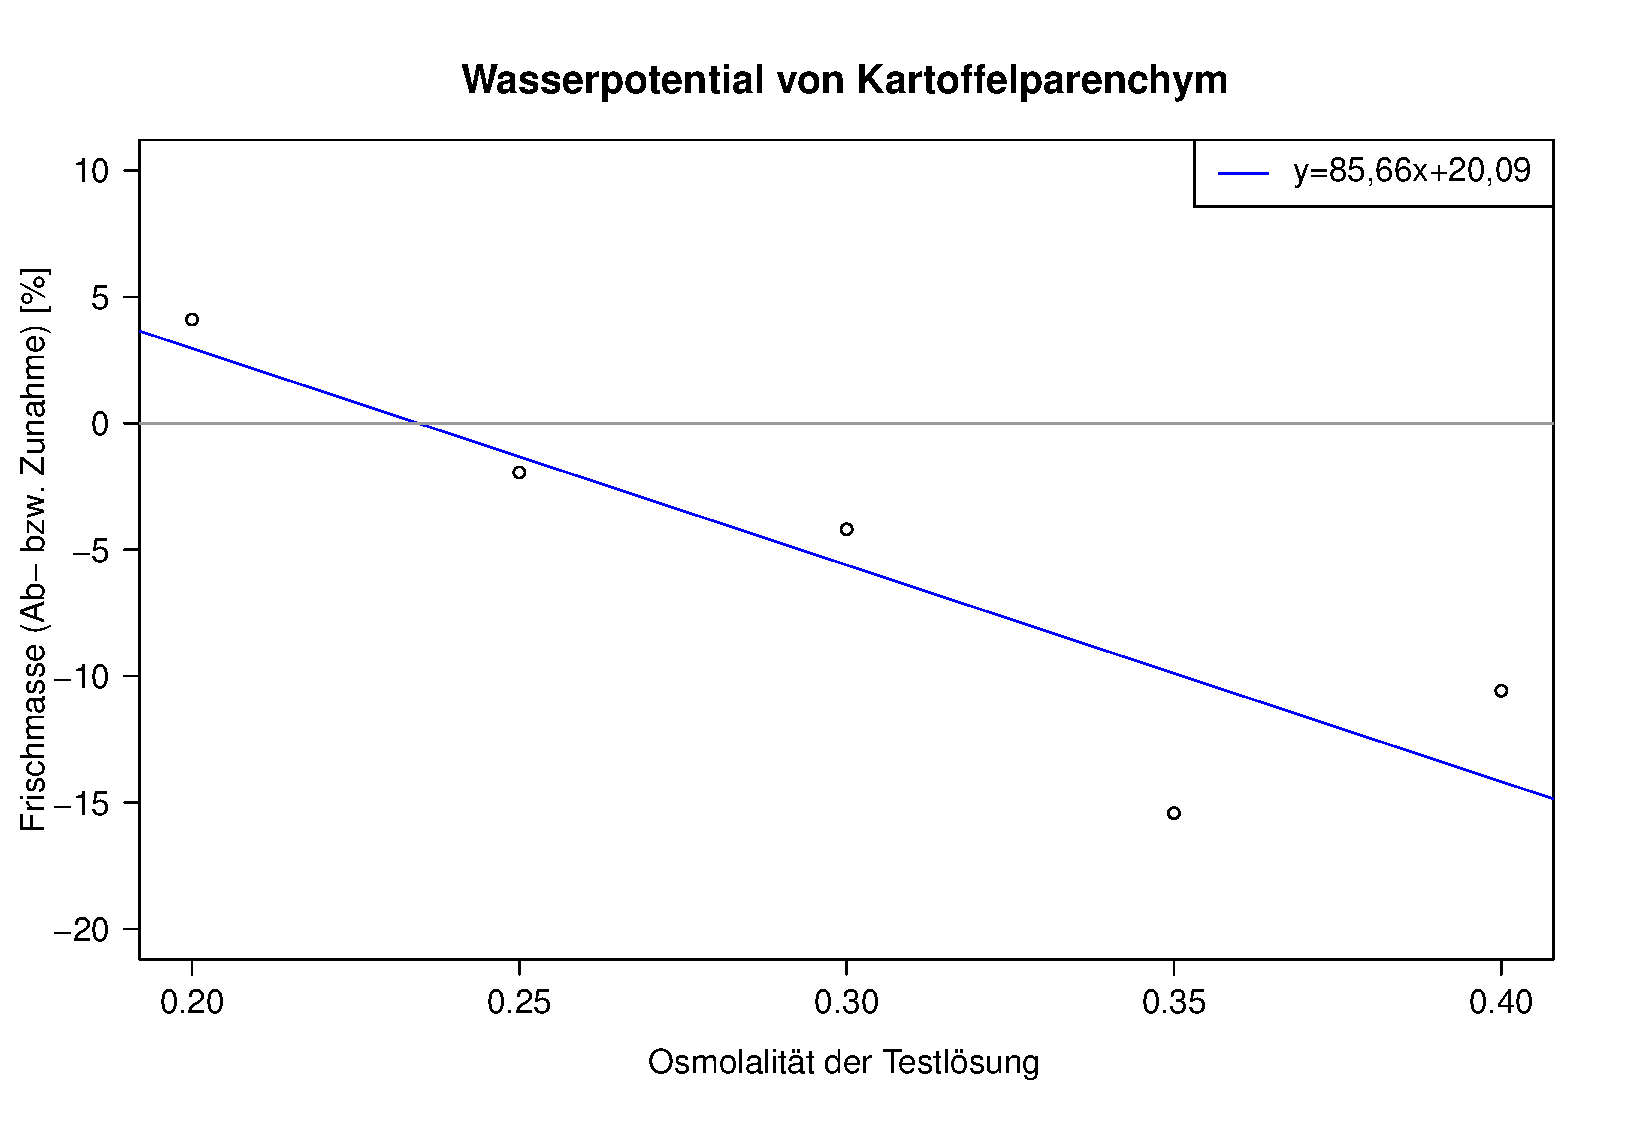
\includegraphics[width=1.0\textwidth]{Abbildungen/Rplot01}
\caption{Abhhängigkeit der Ab- bzw. Zunahme der Masse von der Osmolalität von \textit{Solanum Tuberosum}. Die Regressionsgerade zeigt eine deutliche Tendenz.}
\label{v1}
\end{figure}
\noindent
Mit Hilfe einer Regressionsgerade, die durch die Gleichung
\begin{equation}
y= -85,66x+20,09 \label{regrres}
\end{equation}
beschrieben wird, kann die Konzentration, bei der keine Ab- bzw. Zunahme der Masse stattfindet, berechnet werden. Durch umstellen von (\ref{regrres}) ergibt sich ein Wert von
\begin{equation}
x=0,23 \textrm{~Mol}
\end{equation}
Da eine Lösung im Gleichgewicht mit ihrer Umgebung keinen hydrostatischen Druck aufweist, folgt aus
\begin{equation}
\Psi_W=\Psi_P+\Psi_S
\end{equation}
mit $\Psi_P=0$, dass das Wasserpotential $\Psi_W$ dem osmotischen Potential $\Psi_S$ \textbf{der Saccharo\-se-Lösung} entspricht \citep[vgl.][S. 261]{strasburger_lehrbuch_2012}.
Mit Gleichung (\ref{hoff})
kann daher das Wasserpotential $\Psi_W$ für $c=x=0,23 \textrm{~Mol}$ berechnet werden:
\begin{equation}
\Psi_W=-0,23 \textrm{~Mol} \cdot 8,314 \textrm{~J}\cdot\textrm{K}^{-1}\cdot \textrm{mol}^{-1}\cdot 295 K=-0,56 \textrm{~MPa}
 \end{equation}
Somit beträgt das Wasserpotenzial der untersuchten Gewebeproben -0,56 MPa.
\subsection*{Osmotisches Potential}
Die Messung mit dem Osmometer ergab einen Wert von 346 mOsm/kg. Durch die Verhältnisgleichung
\begin{equation}
\dfrac{-24,8 \cdot 10^5 \textrm{~Pa}}{1 \textrm{~Osm} } = \dfrac{x}{0,346 \textrm{~Osm}}
\end{equation}
lässt sich das osmotische Potential \textbf{des Zellinhalts} berechnen:
\begin{equation}
x = \dfrac{-24,8 \cdot 10^5 \textrm{~Pa} \cdot 0,346 \textrm{~Osm}}{1 \textrm{~Osm} } = -0,858 \textrm{~MPa}
\end{equation}
Mit dem Ergebnis der Kompensationsmethode lässt sich das Druckpotential (\textbf{Turgor}) berechnen:
\begin{equation}
\Psi_p=\Psi_W-\Psi_S=-0,56 \textrm{~MPa} - (-0,86 \textrm{~MPa})= 0,3 \textrm{~MPa}
\end{equation}
%
\section*{Diskussion}
Die erhaltenen Ergebnisse entsprechen den Erwartungen und werden durch die gängige Literatur abgedeckt \citep[vgl.][S. 54]{schopfer_pflanzenphysiologie_2010}. Die ermittelte Regressionsgerade zeigt eine lineare Abnahme, die theoretisch so zu erwarten gewesen ist. 

Wird pflanzliches Gewebe in eine Lösung getaucht, derren Wasserpotenzial \textit{höher} als das der Zellen in dem Gewebe ist, fließt Wasser in diese Zellen hinein. Somit nimmt die Masse des Gewebes zu. Wird das Gewebe in eine Lösung gegeben, derren Wasserpotential \textit{niedriger} als das des Gewebes ist, fließt Wassser aus den Zellen heraus und die Masse nimmt ab. Abbildung \ref{v1} veranschaulicht dieses Phänomen. 

Fehler könnten beim Ansetzen der Verdünnungsreihe enstanden sein. Des Weiteren sind die
Messungenauigkeiten der verwendeteten Pipetten zu berücksichtigen. 
\bibliographystyle{agsm}
\bibliography{pflaphy}
\end{document}